\section{Experimental}
 

In order to determine the tire characteristics of the scaled vehicle, a good testbed is necessary. In this section the experimental setup used to gather the data needed for determining the tire characteristic is discussed.\\
The experimental setup consists of a modified scaled RC car with an on board IMU and a tachometer on each wheel. Moreover, a motion capture system or MoCap was used to provide millimeter precision locating. 

The scaled RC car is a Losi TEN Rally-X. It is a 1:10 scale car with 4WD.  
Each wheel was fitted with it\textquotesingle s own hall effect sensor which generates a pulse every time one of the 24 magnets inside the rim passes it. Furthermore, a set of costum 3D printed wheels were fitted with 24 magnets inside to generate the tacho signal.  Finally, the car\textquotesingle s suspension is replaced with stiff turnbuckle rods to eliminate the degrees of freedom of roll and pitch, to meet the assumptions of the Bicycle model.

\begin{figure}
  \centering
    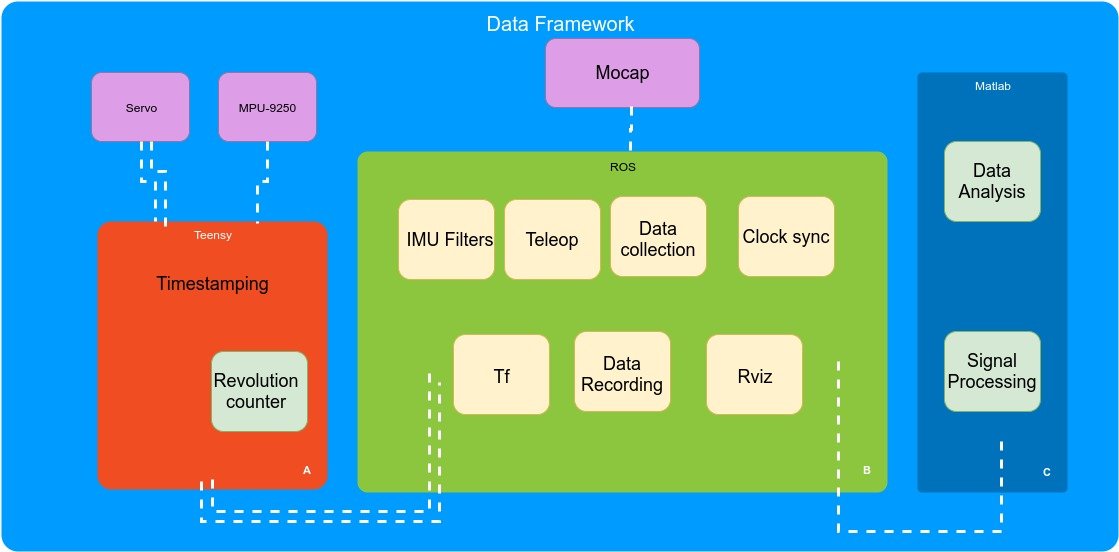
\includegraphics[scale=0.22]{figure/DataFramework}
  \caption{Data acquisition framework}
  \label{fig:DonutFramework} 
\end{figure}

Data acquisition was done using a ROS (Robot Operating System) based system. The sensors were read using a Teensy 3.6 protyping board running a costum ROSserial node, connected to a Raspberry pi 3b running ROS. The MoCap connected to the system utilizig the labs Wi-Fi network. Further communication was done using a self written ROS package. After data collection further processing was done using Matlab.Figure
\ref{fig:DonutFramework} further eleborates the Data acquisition framework

The experiments that we conducted can be classified into three groups. The first set of experiments are the ones on the straight (longitudinal motion). During these we accelerated and braked while driving straight ahead. The second set are the steady state cornering experiments (lateral motion). Steady state cornering means cornering at a constant longitudinal velocity and constant steering angle. The first group of experiments focuses on longitudinal forces and slip ratios, while the second group focuses on lateral forces and slip angles. The tests were separated in order to distinguish longitudinal and lateral motion (Recommendation Barys Shyrokau). Finally, the third set of experiments are of combined motion. These tests take both lateral and longitudinal motion into account. 
	Variables of the tests are acceleration/deceleration for longitudinal motion, longitudinal velocity and steering angle for lateral motion, and these three combined for  combined motion. The variables were slightly increased each experiment in order to determine the \textquotesingle borderline\textquotesingle  between linear and nonlinear behaviour is. 

